\documentclass{article}

\usepackage[english, russian]{babel}
\usepackage{geometry}
\usepackage{graphicx}
\usepackage{listings}
\usepackage{xcolor}
\usepackage[14pt]{extsizes}
\usepackage{amsmath}
\usepackage{setspace}
\usepackage{multirow}
\usepackage{tocloft}
\usepackage{indentfirst} 
\usepackage{lipsum}
\usepackage{caption}
\usepackage{cmap}
\usepackage[utf8]{inputenc}
\usepackage[T2A]{fontenc}

\captionsetup[figure]{name={Рисунок},labelsep=endash}
\captionsetup[table]{singlelinecheck=false, labelsep=endash}

\renewcommand{\cftsecleader}{\cftdotfill{\cftdotsep}}
\geometry{pdftex, left = 3cm, right = 1cm	, top = 2cm, bottom = 2cm}
\onehalfspacing

\setlength{\parindent}{1,25cm}
\lstdefinestyle{lst}{
	basicstyle=\footnotesize\ttfamily,
	frame=single,
	tabsize=4,	
	breaklines=true
}

\DeclareCaptionLabelSeparator{line}{\ --\ }
\DeclareCaptionFont{white}{\color{white}}
\DeclareCaptionFormat{listing}{\colorbox[cmyk]{0.43,0.35,0.35,0.01}{\parbox{\textwidth}{\hspace{15pt}#1#2#3}}}
\captionsetup[lstlisting]{
	singlelinecheck=false,
	labelsep=line
}

\begin{document}
\begin{titlepage}
	\newgeometry{pdftex, left=2cm, right=2cm, top=2.5cm, bottom=2.5cm}
	\fontsize{12pt}{12pt}\selectfont
	\noindent\begin{tabular}{|c|c|}	\hline
	\noindent\begin{minipage}{0.15\textwidth}
		
\includegraphics[width=\linewidth]{tools/logo}
	\end{minipage} &
	\noindent\begin{minipage}{0.85\textwidth}\centering
		\textbf{\newline Министерство науки и высшего образования Российской Федерации}\\
		\textbf{Федеральное государственное бюджетное образовательное учреждение высшего образования}\\
		\textbf{«Московский государственный технический университет имени Н.Э.~Баумана}\\
		\textbf{(национальный исследовательский университет)»}\\
		\textbf{(МГТУ им. Н.Э.~Баумана)}
	\end{minipage} \\
	\hline	\end{tabular}\newline\newline\newline
	\noindent ФАКУЛЬТЕТ \underline{«Информатика и системы управления»} \newline\newline
	\noindent КАФЕДРА \underline{«Программное обеспечение ЭВМ и информационные технологии»}\newline\newline\newline\newline\newline\newline

	\noindent\begin{minipage}{1.0\textwidth}\centering
		\Large\textbf{   ~~~ Лабораторная работа №2}\newline
		\textbf{по дисциплине «Архитектура ЭВМ»}\newline\newline\newline\newline\newline
	\end{minipage}

	\noindent\textbf{Тема} \underline{Изучение принципов работы микропроцессорного ядра RISC-V}
\newline\newline
	\textbf{Студент} \underline{Пантелеев Василий Максимович}\newline\newline
	\textbf{Группа} \underline{ИУ7-52Б}\newline\newline
	\textbf{Преподаватель} \underline{Калитвенцев М.П., Попов А.Ю.}
	
	\begin{center}
		\vfill
		Москва, \the\year ~г.
	\end{center}
	\restoregeometry
	\clearpage
\end{titlepage}

\section{Введение}
Основной \textbf{целью} работы является ознакомление с принципами функционирования, построения и особенностями 
архитектуры суперскалярных конвейерных микропроцессоров. Дополнительной \textbf{целью} работы является знакомство с 
принципами проектирования и верификации сложных цифровых устройств с использованием языка описания аппаратуры 
SystemVerilog и ПЛИС.

Для достижения поставленных целей в настоящей лабораторной работе используется синтезируемое описание 
микропроцессорного ядра Taiga, реализующего систему команд RV32I семейства RISC-V. Данное описание выполнено на языке 
описания аппаратуры SystemVerilog.

В ходе лабораторной работы используется средство моделирования MentorGraphics Modelsim для моделирования работы 
исследуемого микропроцессора в процессе выполнения программы и наблюдения формы внутренних сигналов.

\section{Задание 1}
\subsection{Исходный текст исследуемой программы}
\begin{lstlisting}[style=lst, caption=Исходный текст исследуемой программы]
.section .text
        .globl _start;
        len = 9
        enroll = 1
        elem_sz = 4

_start:
        la x1, _x
        addi x20, x1, elem_sz*len
        lw x31, 0(x1)
        add x1, x1, elem_sz*1
lp:
        lw x2, 0(x1)
        bltu x2, x31, lt
        add x31, x0, x2 #!
lt:
        add x1, x1, elem_sz*enroll
        bne x1, x20, lp
lp2: j lp2

        .section .data
_x:     .4byte 0x1
        .4byte 0x2
        .4byte 0x3
        .4byte 0x4
        .4byte 0x5
        .4byte 0x6
        .4byte 0x7
        .4byte 0x8
        .4byte 0x9
\end{lstlisting}

\subsection{Дизассемблированный листинг}
\begin{lstlisting}[style=lst, caption=Дизассемблированный листинг программы]
Disassembly of section .text:

80000000 <_start>:
80000000:	00000097          	auipc	x1,0x0
80000004:	02c08093          	addi	x1,x1,44 # 8000002c <_x>
80000008:	02408a13          	addi	x20,x1,36
8000000c:	0000af83          	lw	x31,0(x1)
80000010:	00408093          	addi	x1,x1,4

80000014 <lp>:
80000014:	0000a103          	lw	x2,0(x1)
80000018:	01f16463          	bltu	x2,x31,80000020 <lt>
8000001c:	00200fb3          	add	x31,x0,x2

80000020 <lt>:
80000020:	00408093          	addi	x1,x1,4
80000024:	ff4098e3          	bne	x1,x20,80000014 <lp>

80000028 <lp2>:
80000028:	0000006f          	jal	x0,80000028 <lp2>

Disassembly of section .data:

8000002c <_x>:
8000002c:	0001                	.insn	2, 0x0001
8000002e:	0000                	.insn	2, 0x
80000030:	0002                	.insn	2, 0x0002
80000032:	0000                	.insn	2, 0x
80000034:	00000003          	lb	x0,0(x0) # 0 <enroll-0x1>
80000038:	0004                	.insn	2, 0x0004
8000003a:	0000                	.insn	2, 0x
8000003c:	0005                	.insn	2, 0x0005
8000003e:	0000                	.insn	2, 0x
80000040:	0006                	.insn	2, 0x0006
80000042:	0000                	.insn	2, 0x
80000044:	00000007          	.insn	4, 0x0007
80000048:	0008                	.insn	2, 0x0008
8000004a:	0000                	.insn	2, 0x
8000004c:	0009                	.insn	2, 0x0009
\end{lstlisting}

\subsection{Псевдокод, поясняющий работу программы}
\begin{lstlisting}[style=lst, caption=pcode]
int main() {
    int _x[] = {0x1, 0x2, 0x3, 0x4, 0x5, 0x6, 0x7, 0x8, 0x9};
    const int len = 9;
    const int enroll = 1;
    const int elem_sz = 4;


    int *x1 = _x;
    int *x20 = _x + len;
    int x31 = *x1;

    x1++;

    while (x1 != x20) {
        int x2 = *x1;

        if (x2 >= x31) {
            x31 = x2;
        }

        x1 += enroll;
    }

    printf("Maximum value: %d\n", x31);

    while (1) {}

    return 0;
}
\end{lstlisting}

\clearpage\section{Задание 2}
\begin{figure}[h]
	\centering
	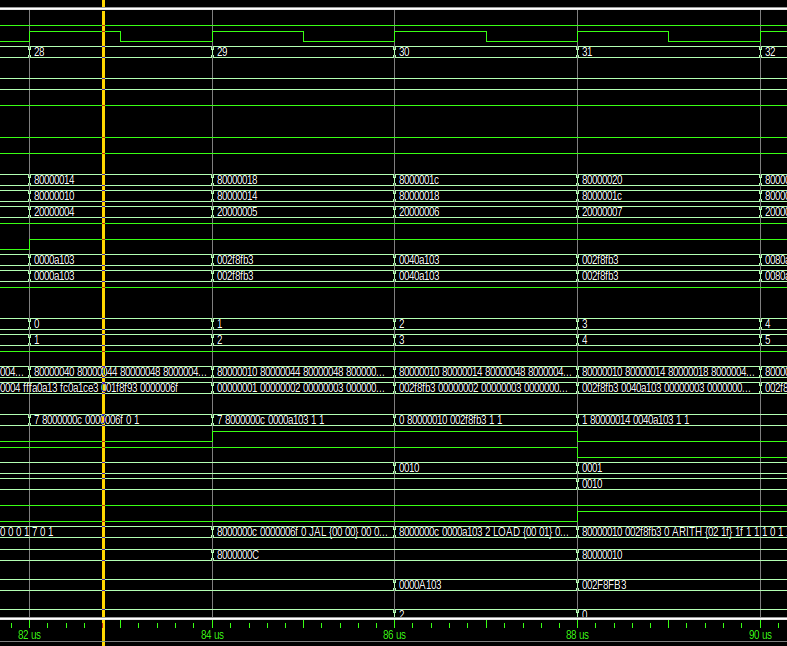
\includegraphics[scale=0.4]{tools/task2}
	\caption{Стадии выборки и диспетчеризации}
\end{figure}

\clearpage\section{Задание 3}
\begin{figure}[h]
	\centering
	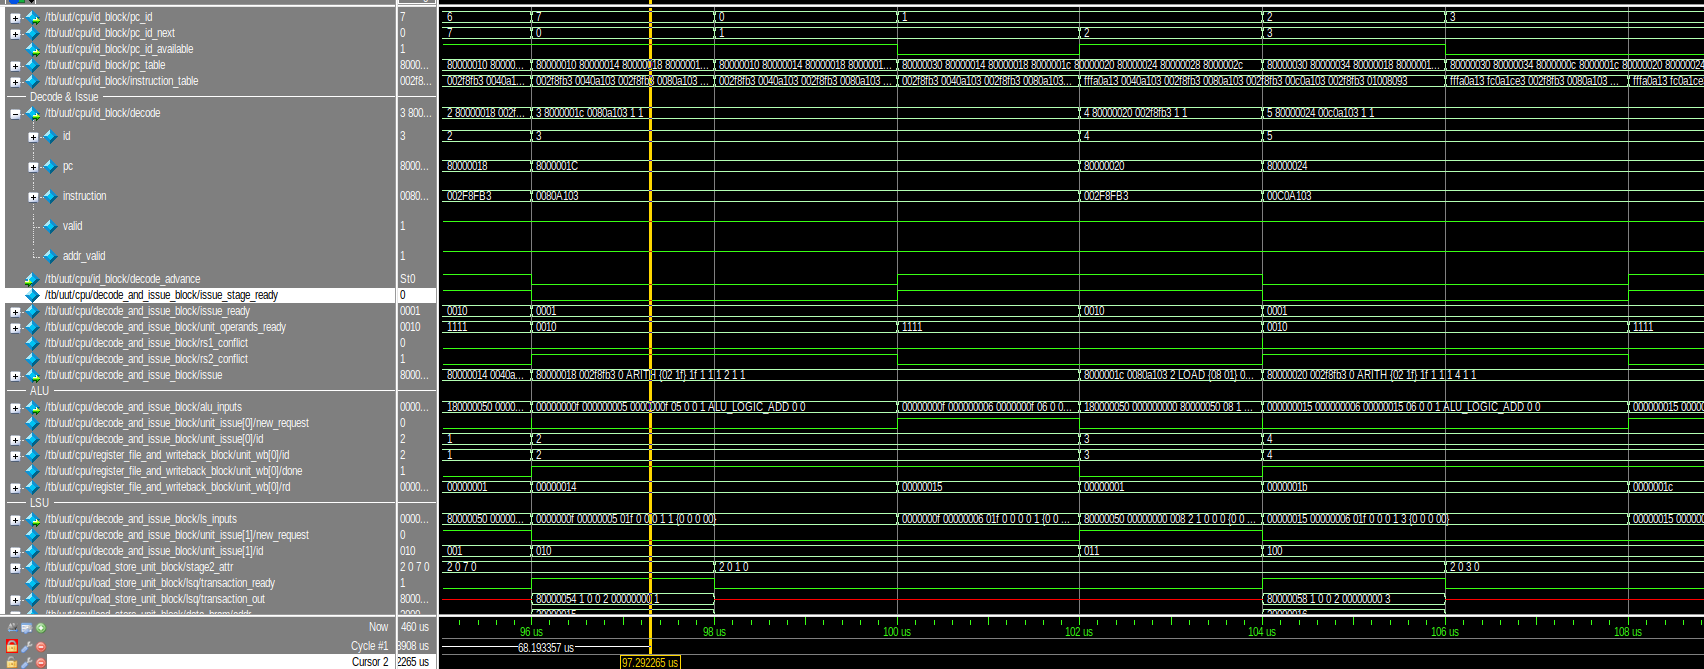
\includegraphics[scale=0.4]{tools/task3}
	\caption{Стадии декодирования и планирования}
\end{figure}

\clearpage\section{Задание 4}
\begin{figure}[h]
	\centering
	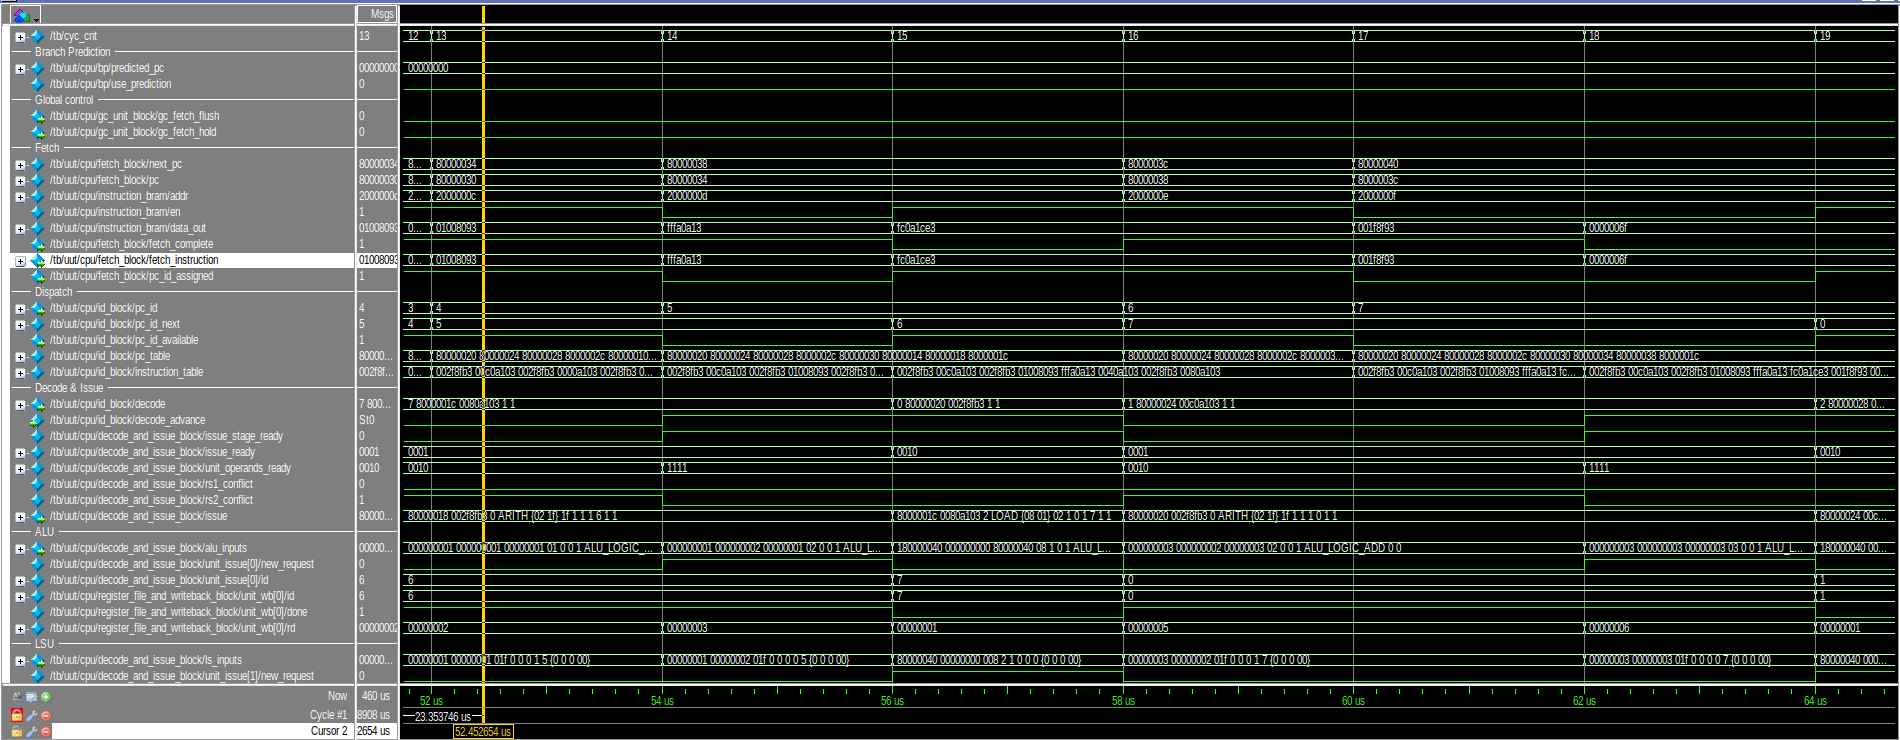
\includegraphics[scale=0.4]{tools/task4}
	\caption{Непосредственное выполнение комманды}
\end{figure}

\clearpage\section{Задание 5}
\subsection{Место, отмеченное решеткой}
\begin{figure}[h]
	\centering
	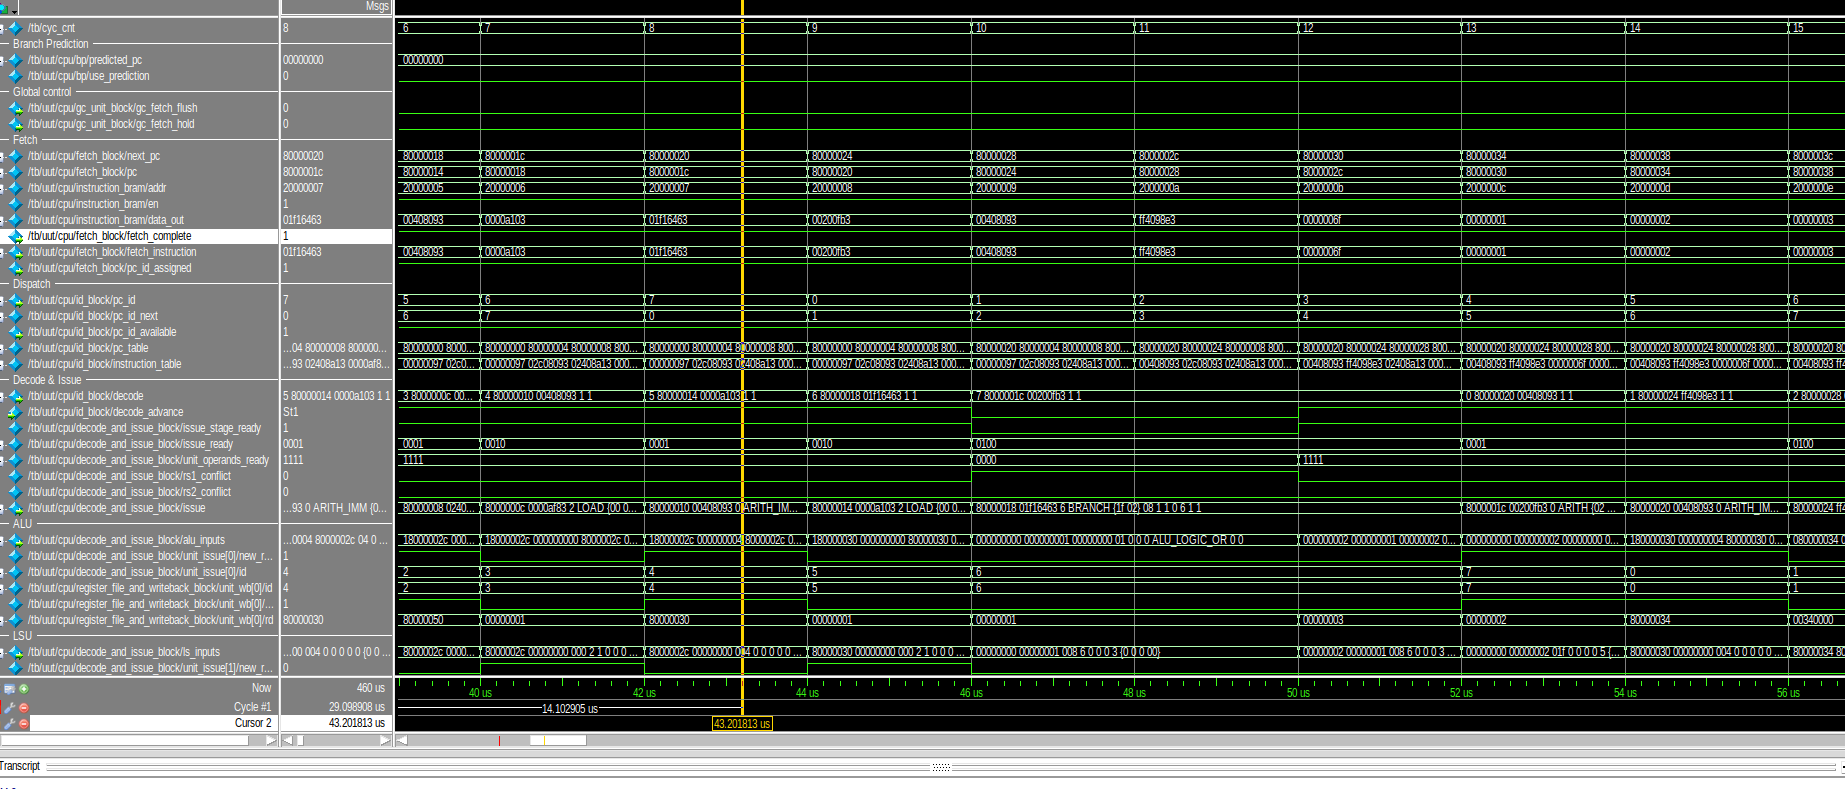
\includegraphics[scale=0.4]{tools/task5_1}
	\caption{Первая итерация команды, отмеченной \#}
\end{figure}

\begin{figure}[h]
	\centering
	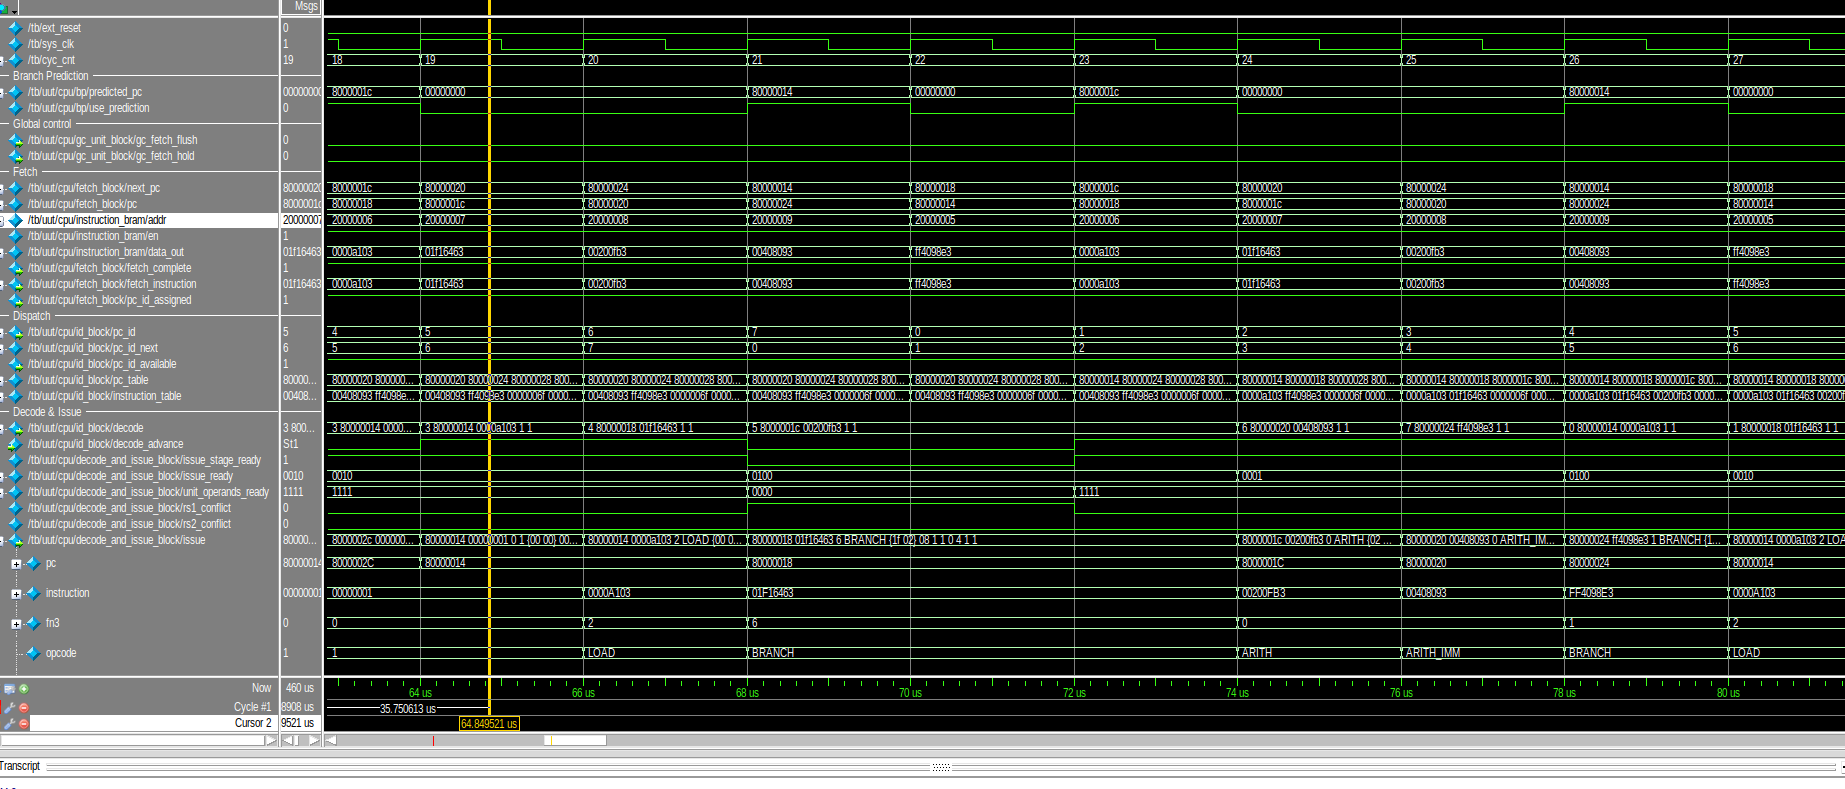
\includegraphics[scale=0.4]{tools/task5_2}
	\caption{Вторая итерация команды, отмеченной \#}
\end{figure}

\begin{figure}[h]
	\centering
	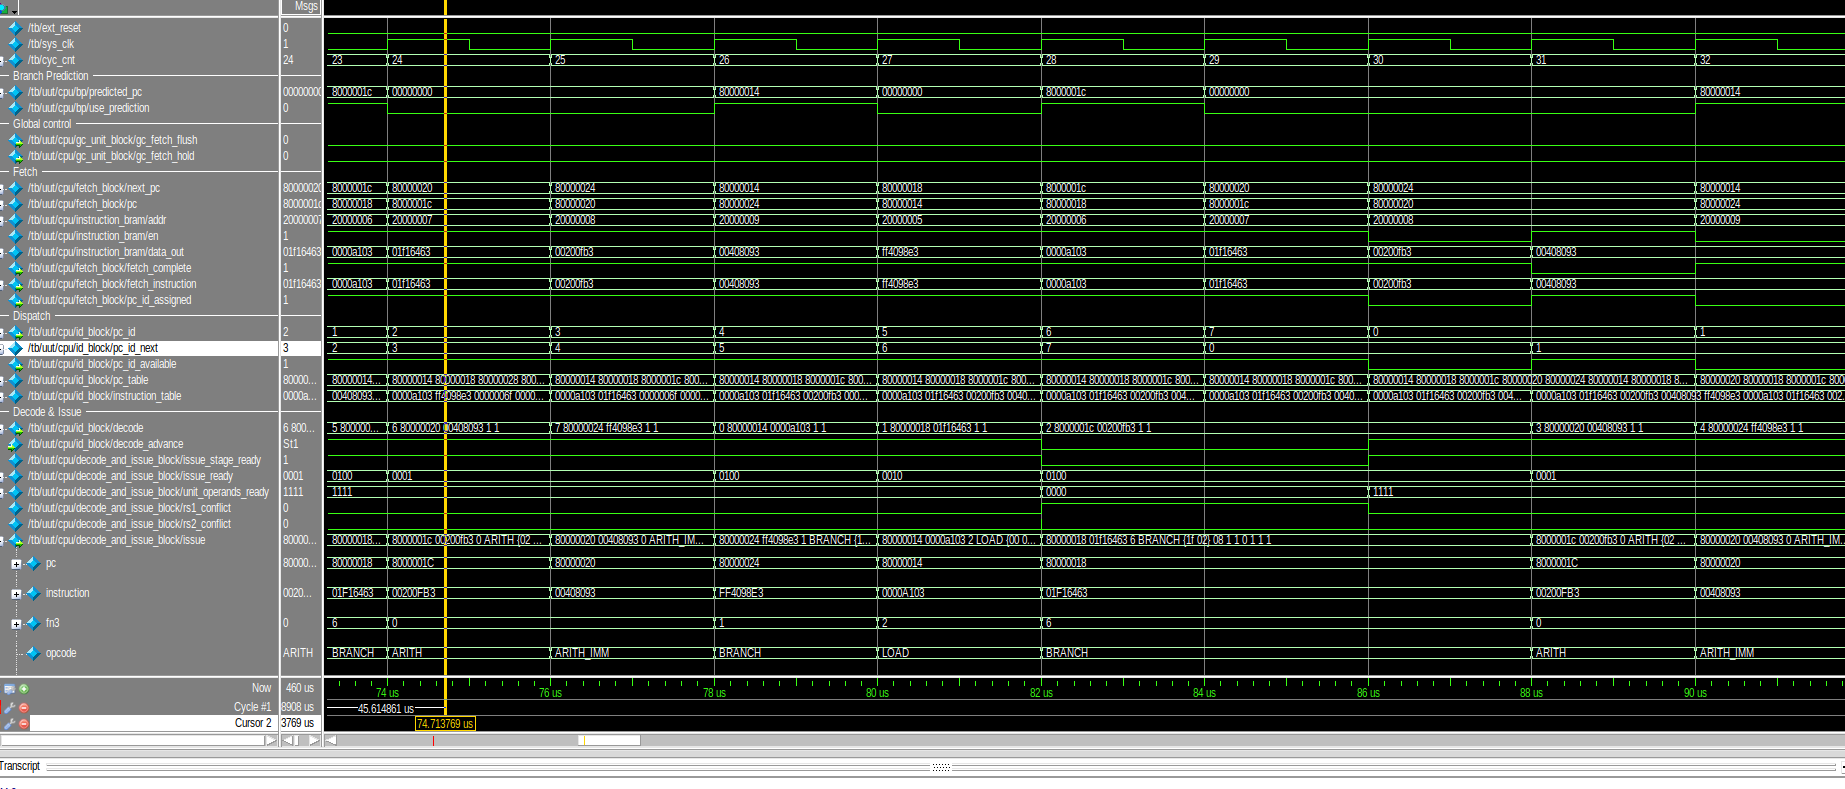
\includegraphics[scale=0.4]{tools/task5_3}
	\caption{Третья итерация команды, отмеченной \#}
\end{figure}

\begin{figure}[h]
	\centering
	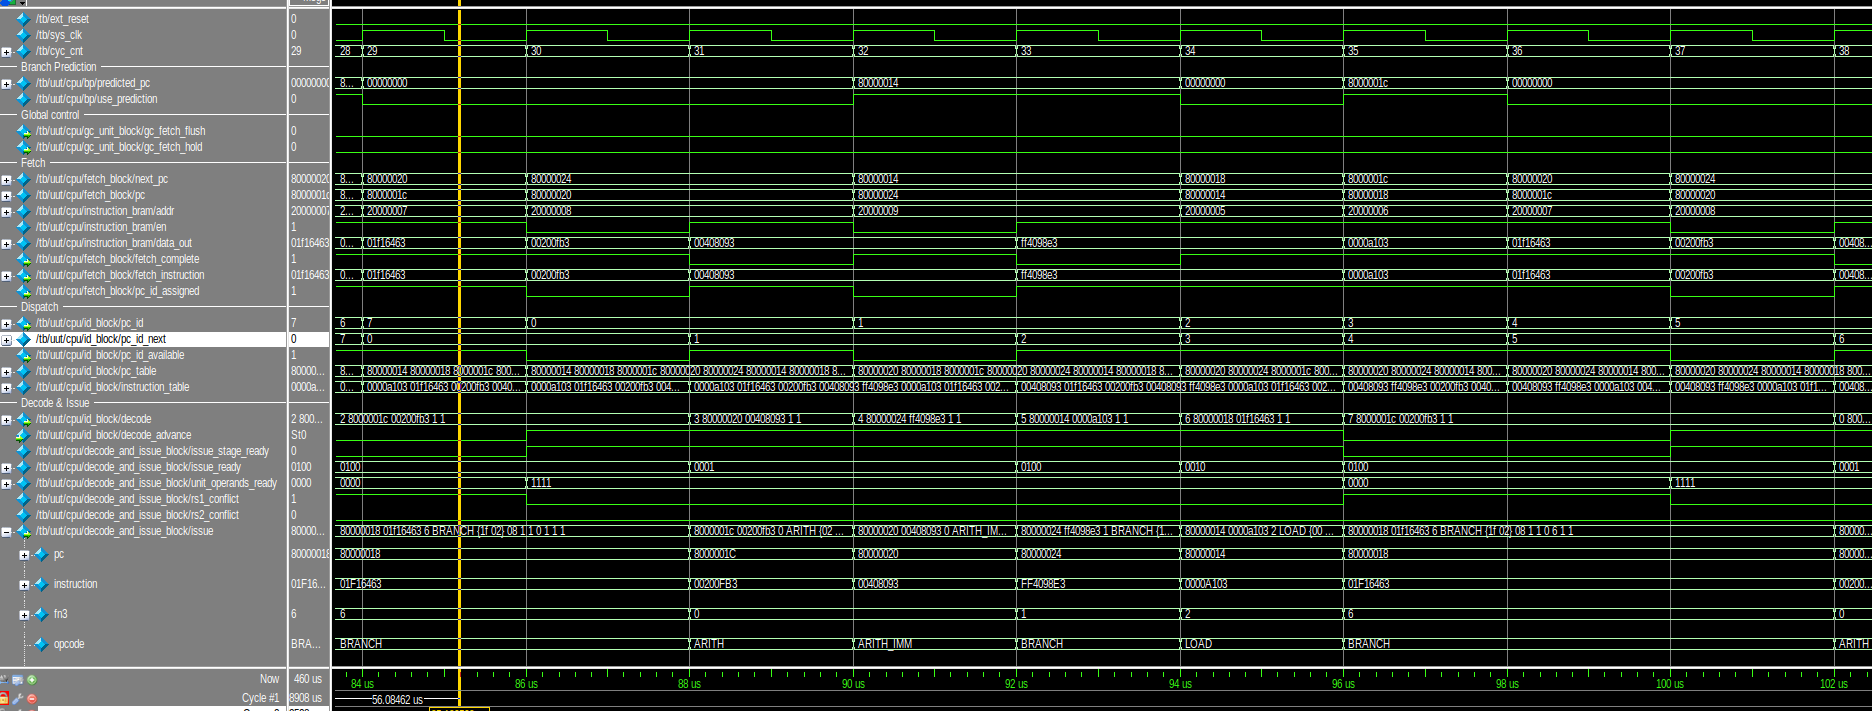
\includegraphics[scale=0.4]{tools/task5_4}
	\caption{Четвертая итерация команды, отмеченной \#}
\end{figure}

\begin{figure}[h]
	\centering
	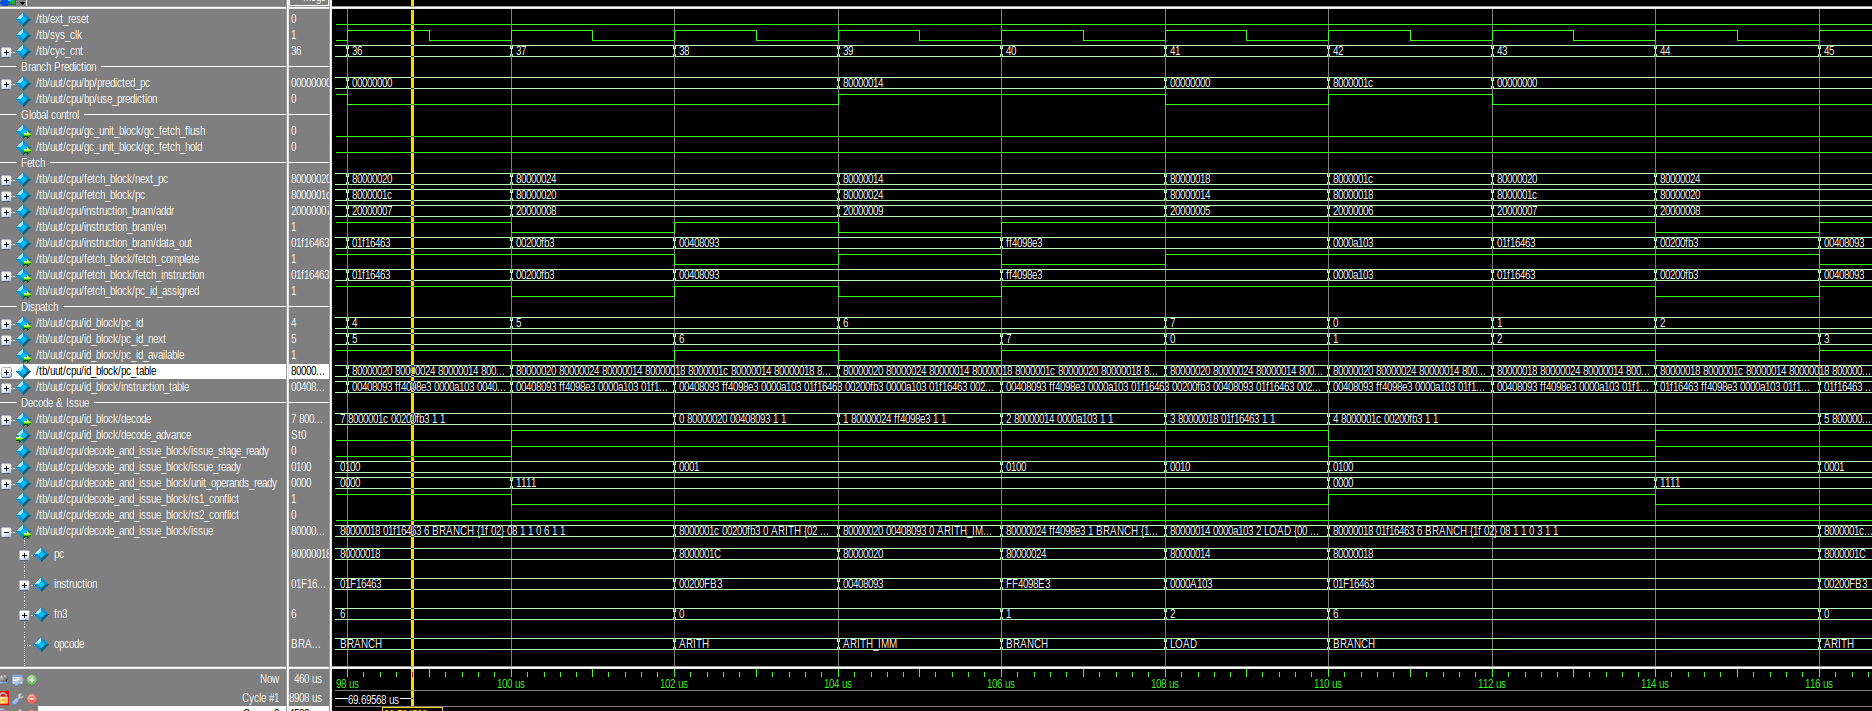
\includegraphics[scale=0.4]{tools/task5_5}
	\caption{Пятая итерация команды, отмеченной \#}
\end{figure}

\begin{figure}[h]
	\centering
	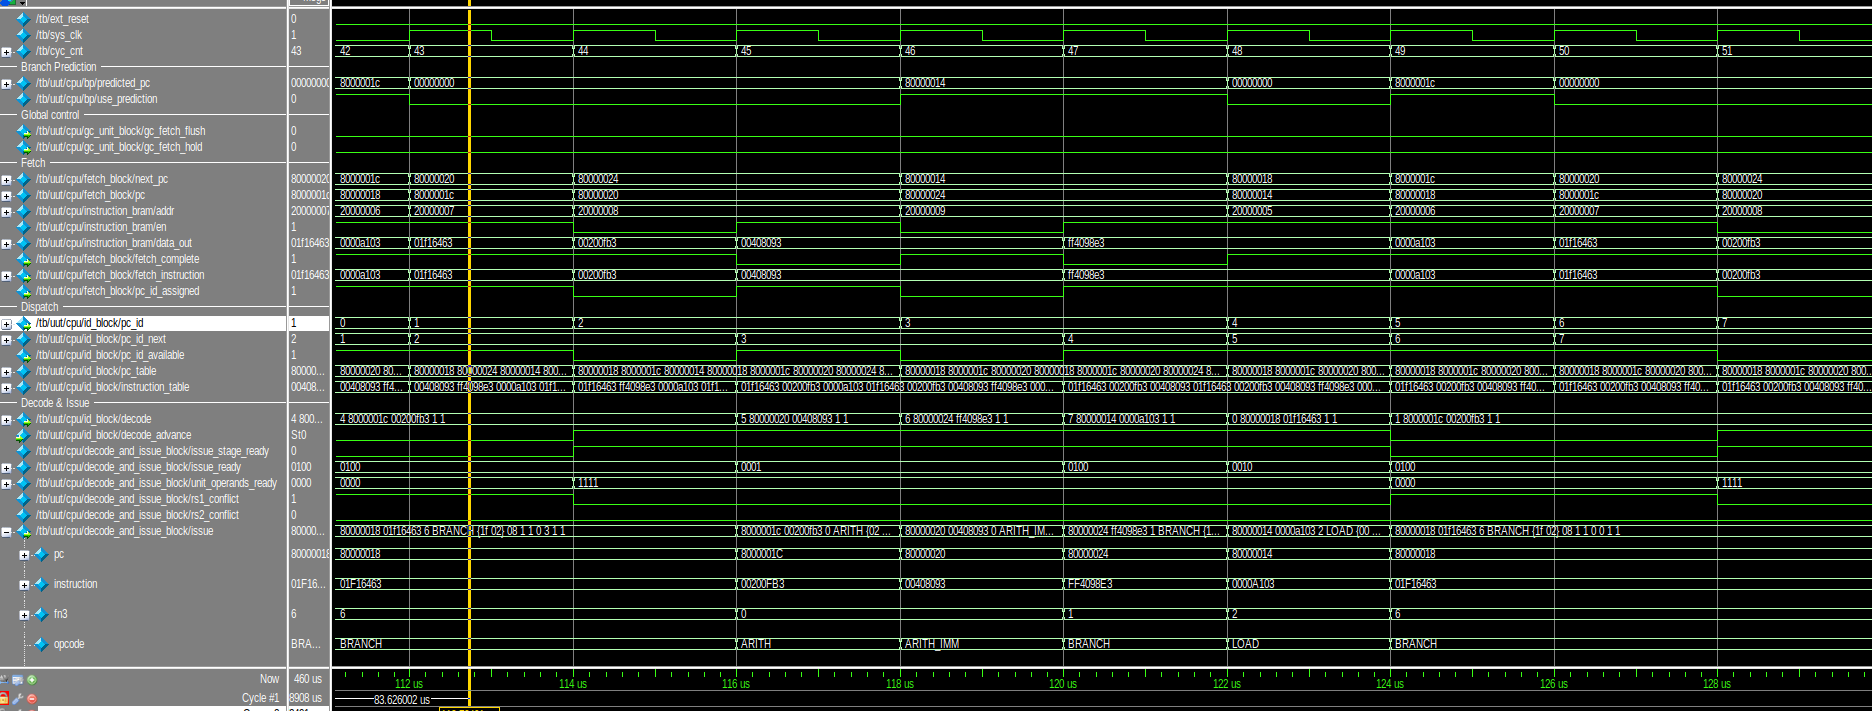
\includegraphics[scale=0.4]{tools/task5_6}
	\caption{Шестая итерация команды, отмеченной \#}
\end{figure}

\begin{figure}[h]
	\centering
	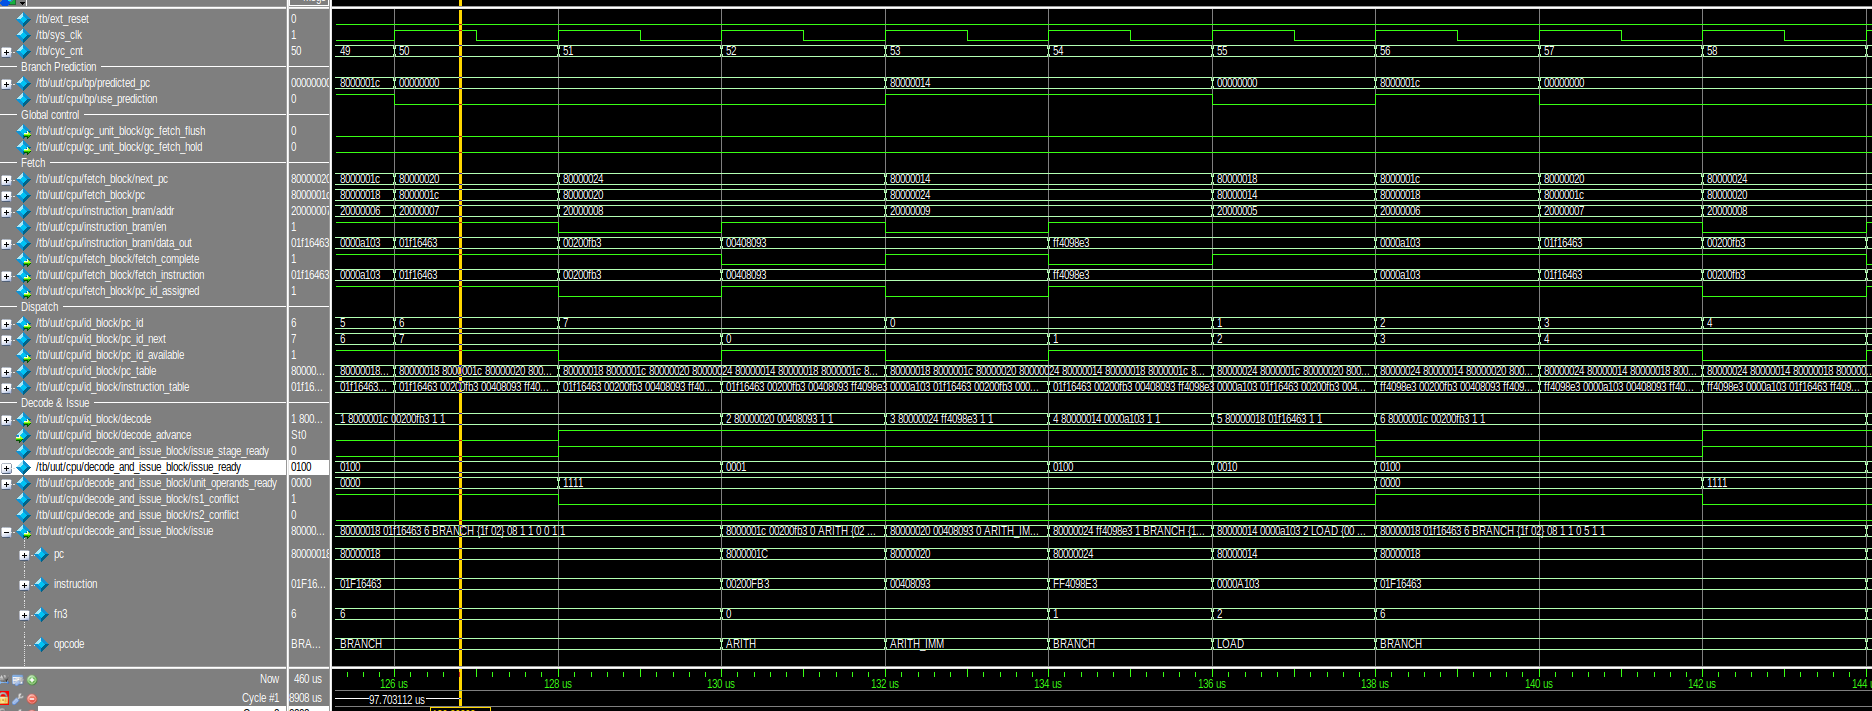
\includegraphics[scale=0.4]{tools/task5_7}
	\caption{Седьмая итерация команды, отмеченной \#}
\end{figure}

\begin{figure}[h]
	\centering
	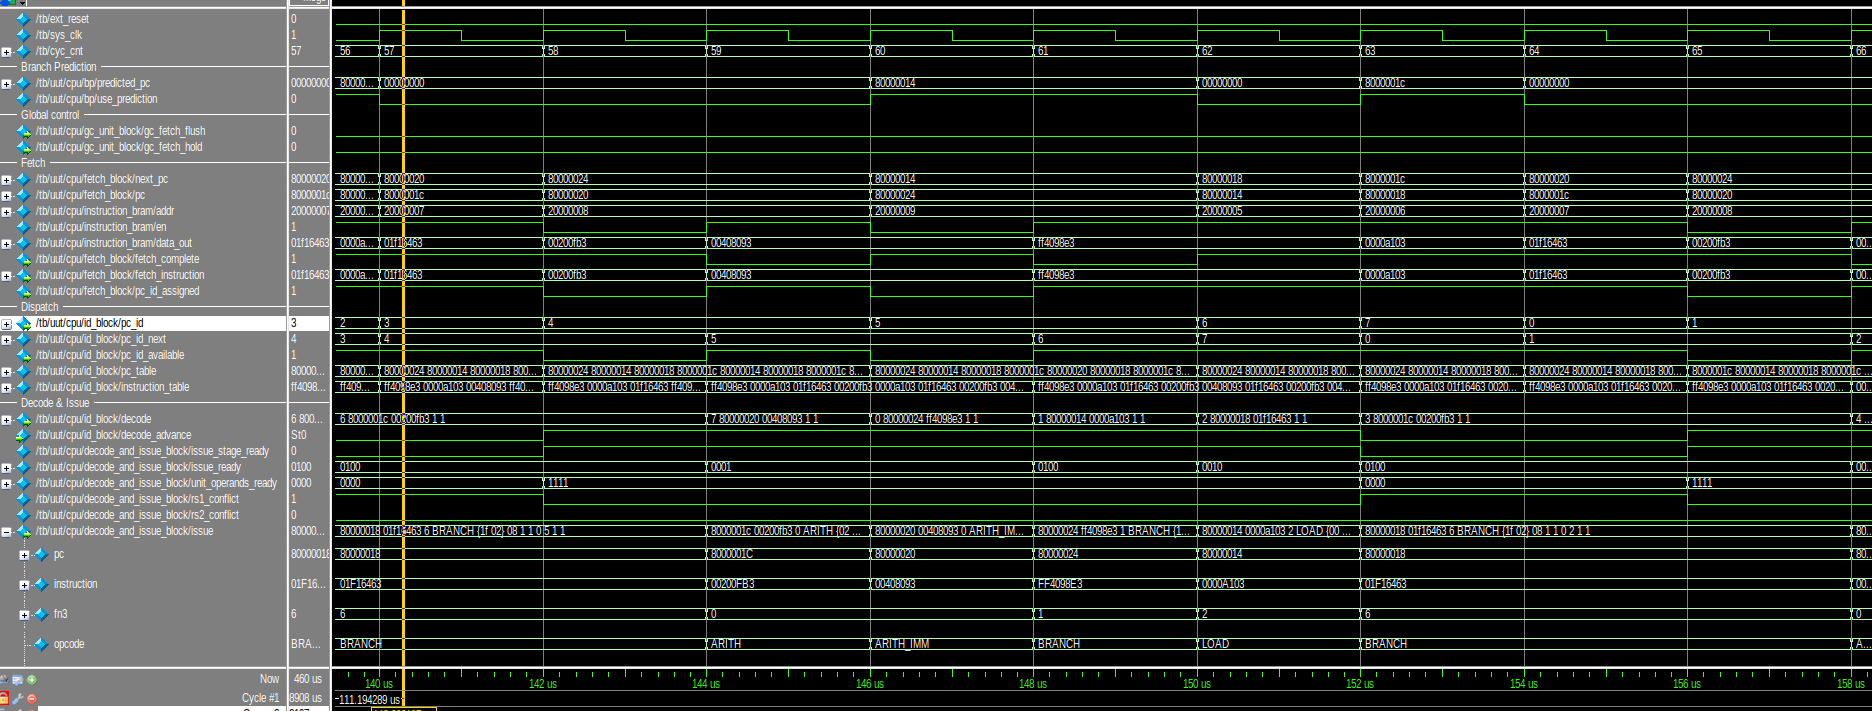
\includegraphics[scale=0.4]{tools/task5_8}
	\caption{Восьмая итерация команды, отмеченной \#}
\end{figure}

\begin{figure}[h]
	\centering
	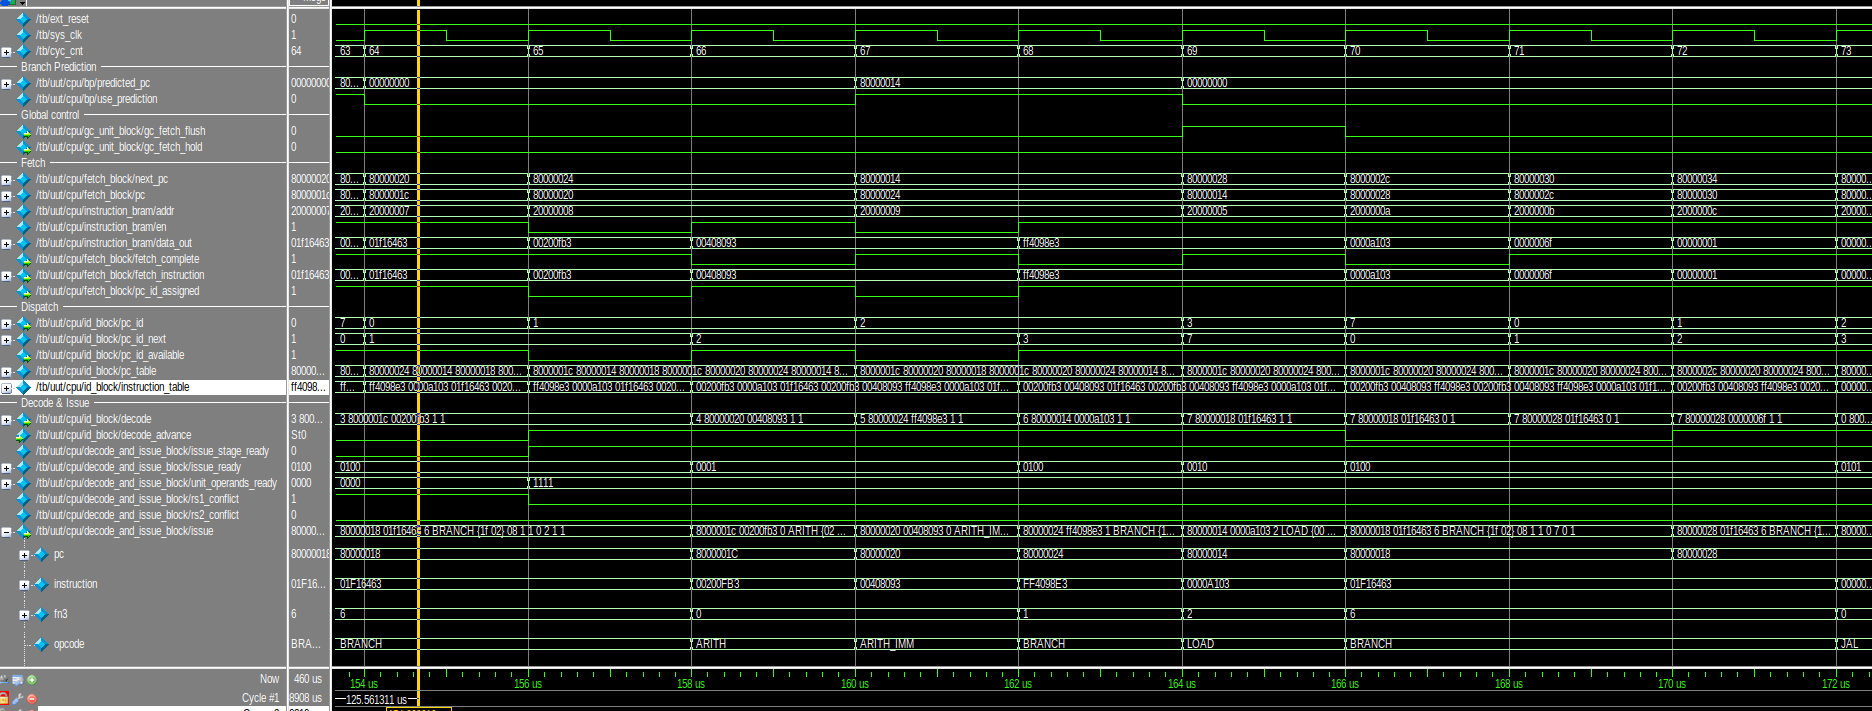
\includegraphics[scale=0.4]{tools/task5_9}
	\caption{Девятая итерация команды, отмеченной \#}
\end{figure}


\clearpage\subsection{Трасса исходной программы}
\begin{figure}[h]
	\centering
	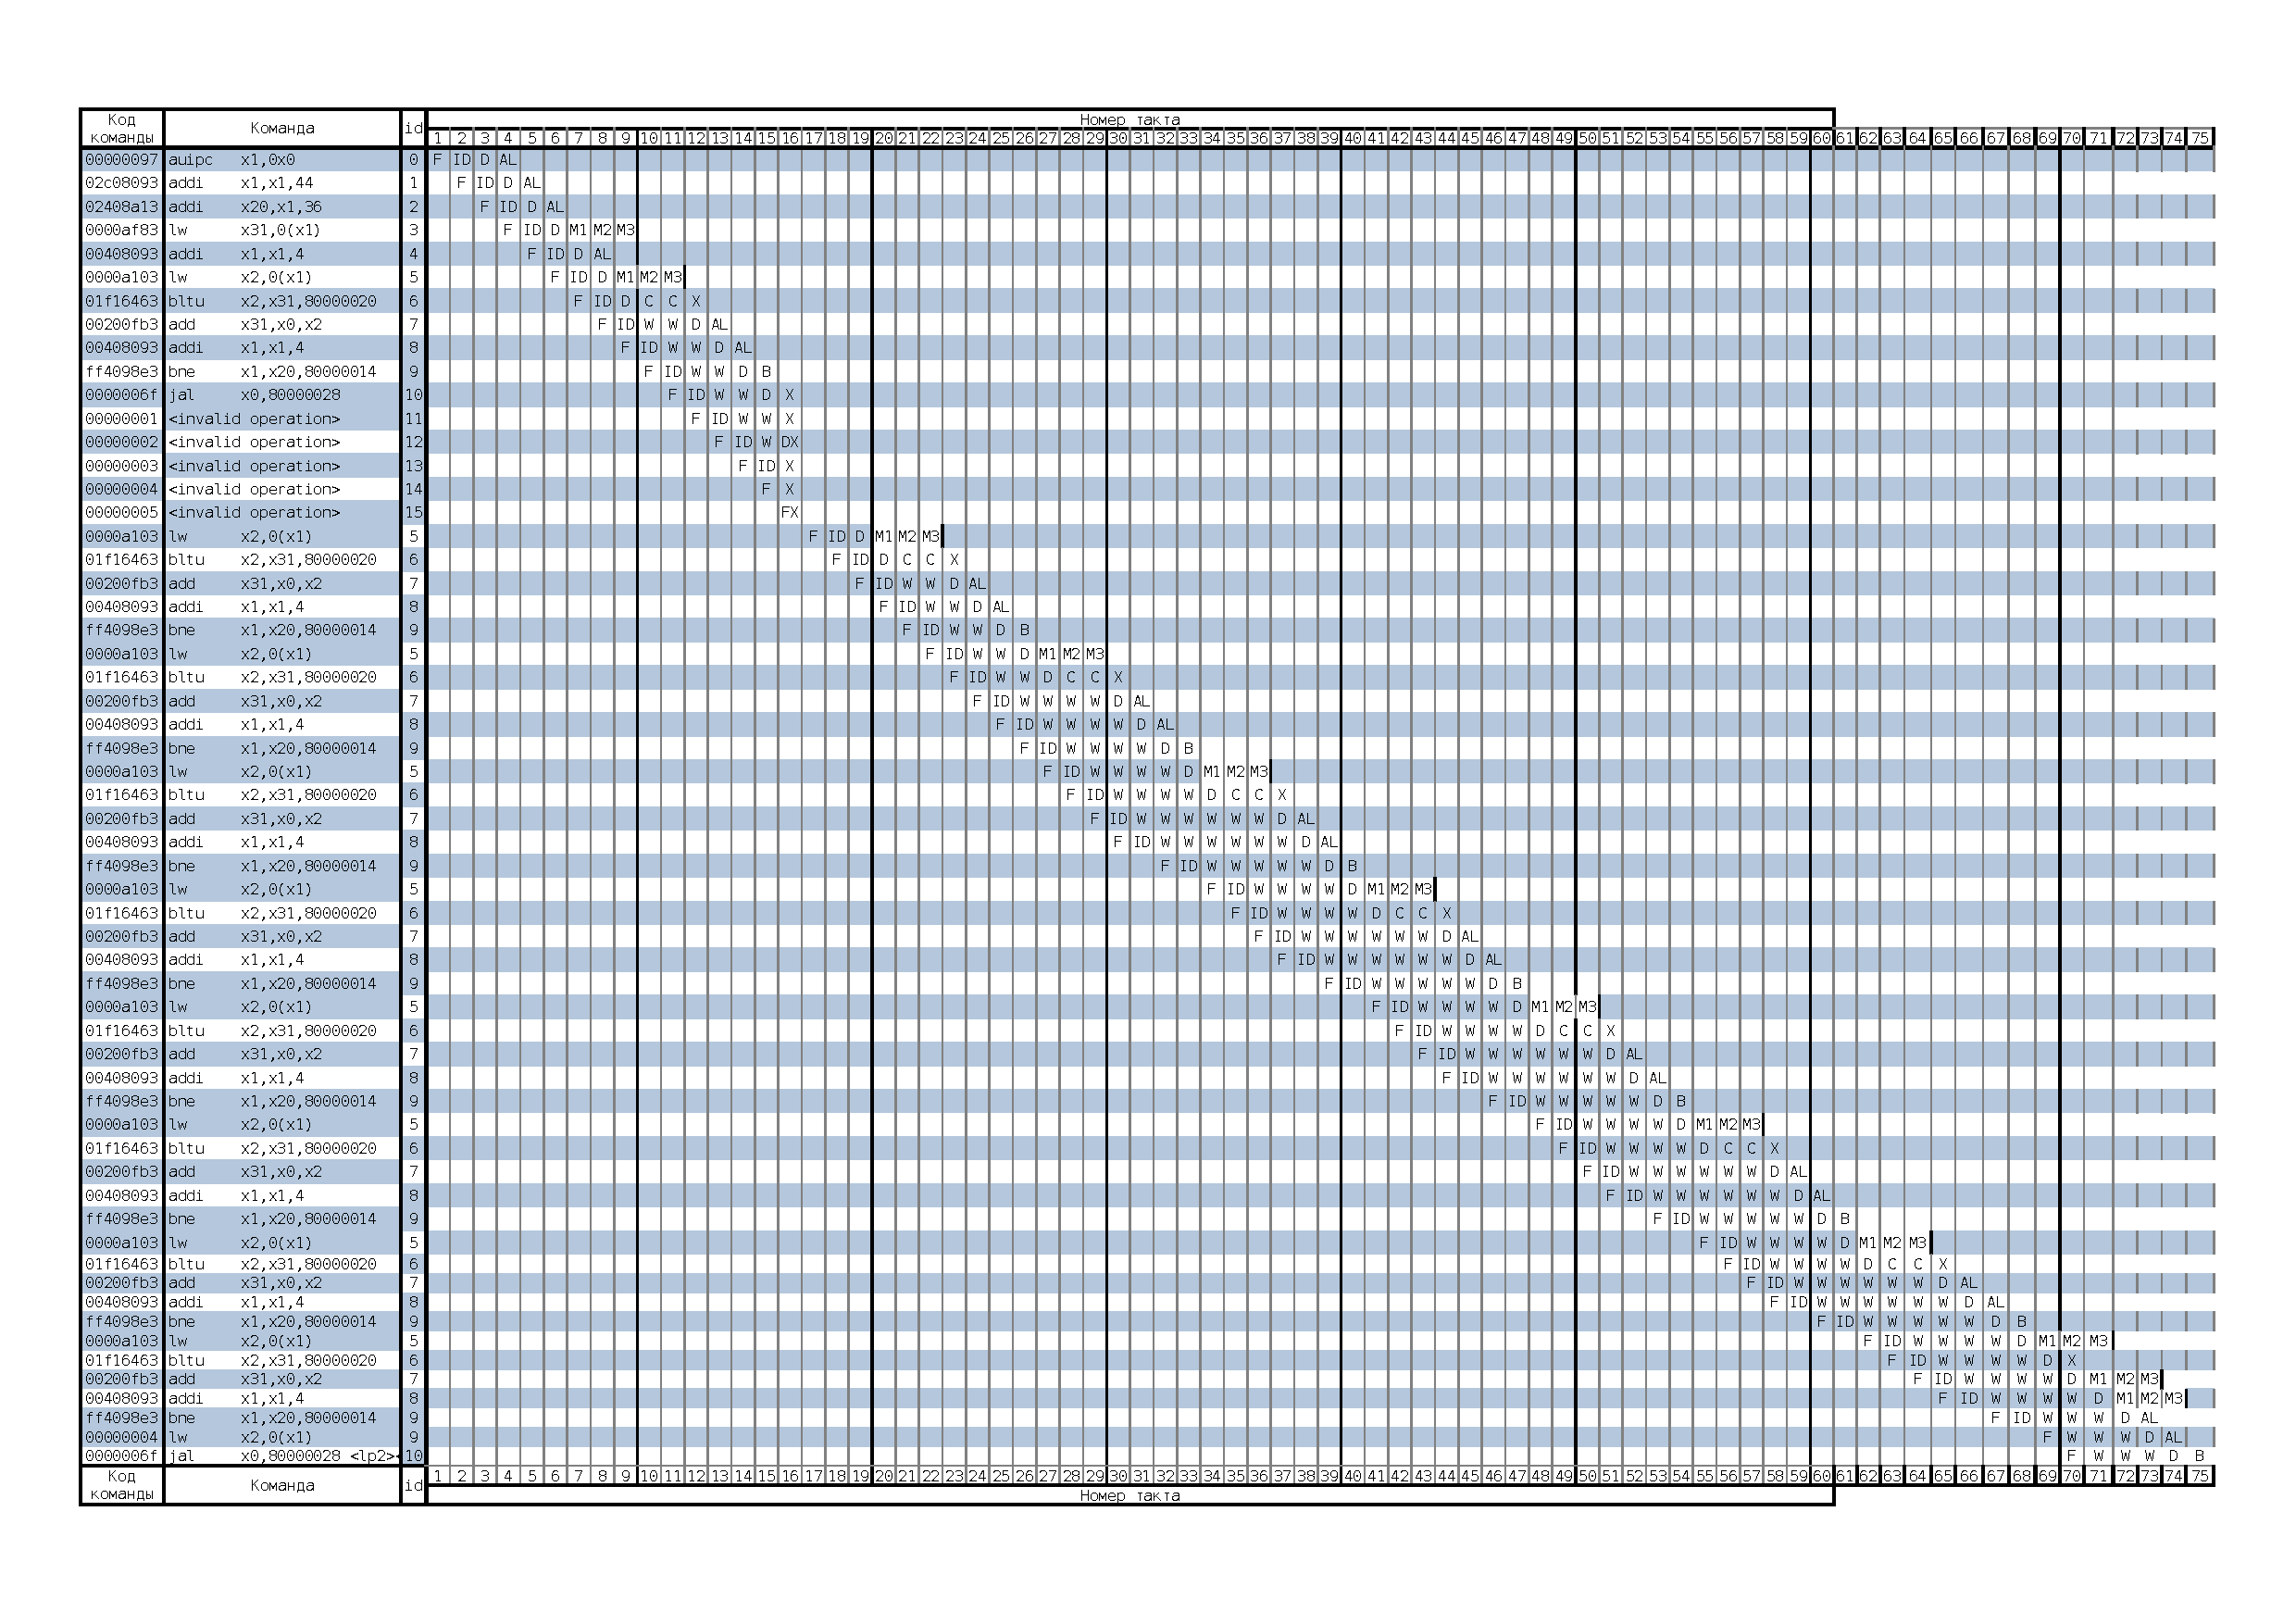
\includegraphics[scale=0.4]{tools/pipeline.pdf}
          \caption{Трасса выполнения неоптимизированной программы}
\end{figure}

\clearpage

Конфликты возникают из-за того, что происходит обращение к регистру, запись в который ещё не была завершена (регистр x2).

Cтрока x1 += enroll (add x1, x1, elem\_sz*enroll) будет выполнена вне зависимости от предшествующих условных переходов, а 
также значение регистра x1 не используется после строки  lw x2, 0(x1) в пределах выполнения тела цикла.

Следовательно, если поместить строку add x1, x1, slem\_sz*enroll сразу после  lw x2, 0(x1), это не повлияет на результат
выполнения программы, зато даст дополнительную задержку в один такт между загрузкой значения в x2 и чтением из него, что 
позволит устранить конфликты.

\clearpage\subsection{Исходной текст оптимизированной программы}
\begin{lstlisting}[style=lst, caption=Исходный текст оптимизированной программы]
        .section .text
        .globl _start;
        len = 9
        enroll = 1
        elem_sz = 4

_start:
    la x1, _x
    addi x20, x1, elem_sz*len
    lw x31, 0(x1)
    add x1, x1, elem_sz*1

lp:
    lw x2, 0(x1)
    add x1, x1, elem_sz*enroll
    nop
    bltu x2, x31, lt
    add x31, x0, x2
lt:
    bne x1, x20, lp

lp2:
    j lp2

.section .data
_x:
    .4byte 0x1
    .4byte 0x2
    .4byte 0x3
    .4byte 0x4
    .4byte 0x5
    .4byte 0x6
    .4byte 0x7
    .4byte 0x8
    .4byte 0x9
\end{lstlisting}

\clearpage\subsection{Дизассемблированный листинг оптимизированной программы}
\begin{lstlisting}[style=lst, caption=Дизассемблированный листинг оптимизированной программы]
Disassembly of section .text:
80000000 <_start>:
80000000:       00000097                auipc   x1,0x0
80000004:       03008093                addi    x1,x1,48 # 80000030 <_x>
80000008:       02408a13                addi    x20,x1,36
8000000c:       0000af83                lw      x31,0(x1)
80000010:       00408093                addi    x1,x1,4

80000014 <lp>:
80000014:       0000a103                lw      x2,0(x1)
80000018:       00408093                addi    x1,x1,4
8000001c:       00000013                addi    x0,x0,0
80000020:       01f16463                bltu    x2,x31,80000028 <lt>
80000024:       00200fb3                add     x31,x0,x2

80000028 <lt>:
80000028:       ff4096e3                bne     x1,x20,80000014 <lp>

8000002c <lp2>:
8000002c:       0000006f                jal     x0,8000002c <lp2>

Disassembly of section .data:

80000030 <_x>:
80000030:       0001                    .insn   2, 0x0001
80000032:       0000                    .insn   2, 0x
80000034:       0002                    .insn   2, 0x0002
80000036:       0000                    .insn   2, 0x
80000038:       00000003                lb      x0,0(x0) # 0 <enroll-0x1>
8000003c:       0004                    .insn   2, 0x0004
8000003e:       0000                    .insn   2, 0x
80000040:       0005                    .insn   2, 0x0005
80000042:       0000                    .insn   2, 0x
80000044:       0006                    .insn   2, 0x0006
80000046:       0000                    .insn   2, 0x
80000048:       00000007                .insn   4, 0x0007
8000004c:       0008                    .insn   2, 0x0008
8000004e:       0000                    .insn   2, 0x
80000050:       0009                    .insn   2, 0x0009
\end{lstlisting}

\clearpage\subsection{Трасса оптимизированной программы}
\begin{figure}[h]
	\centering
	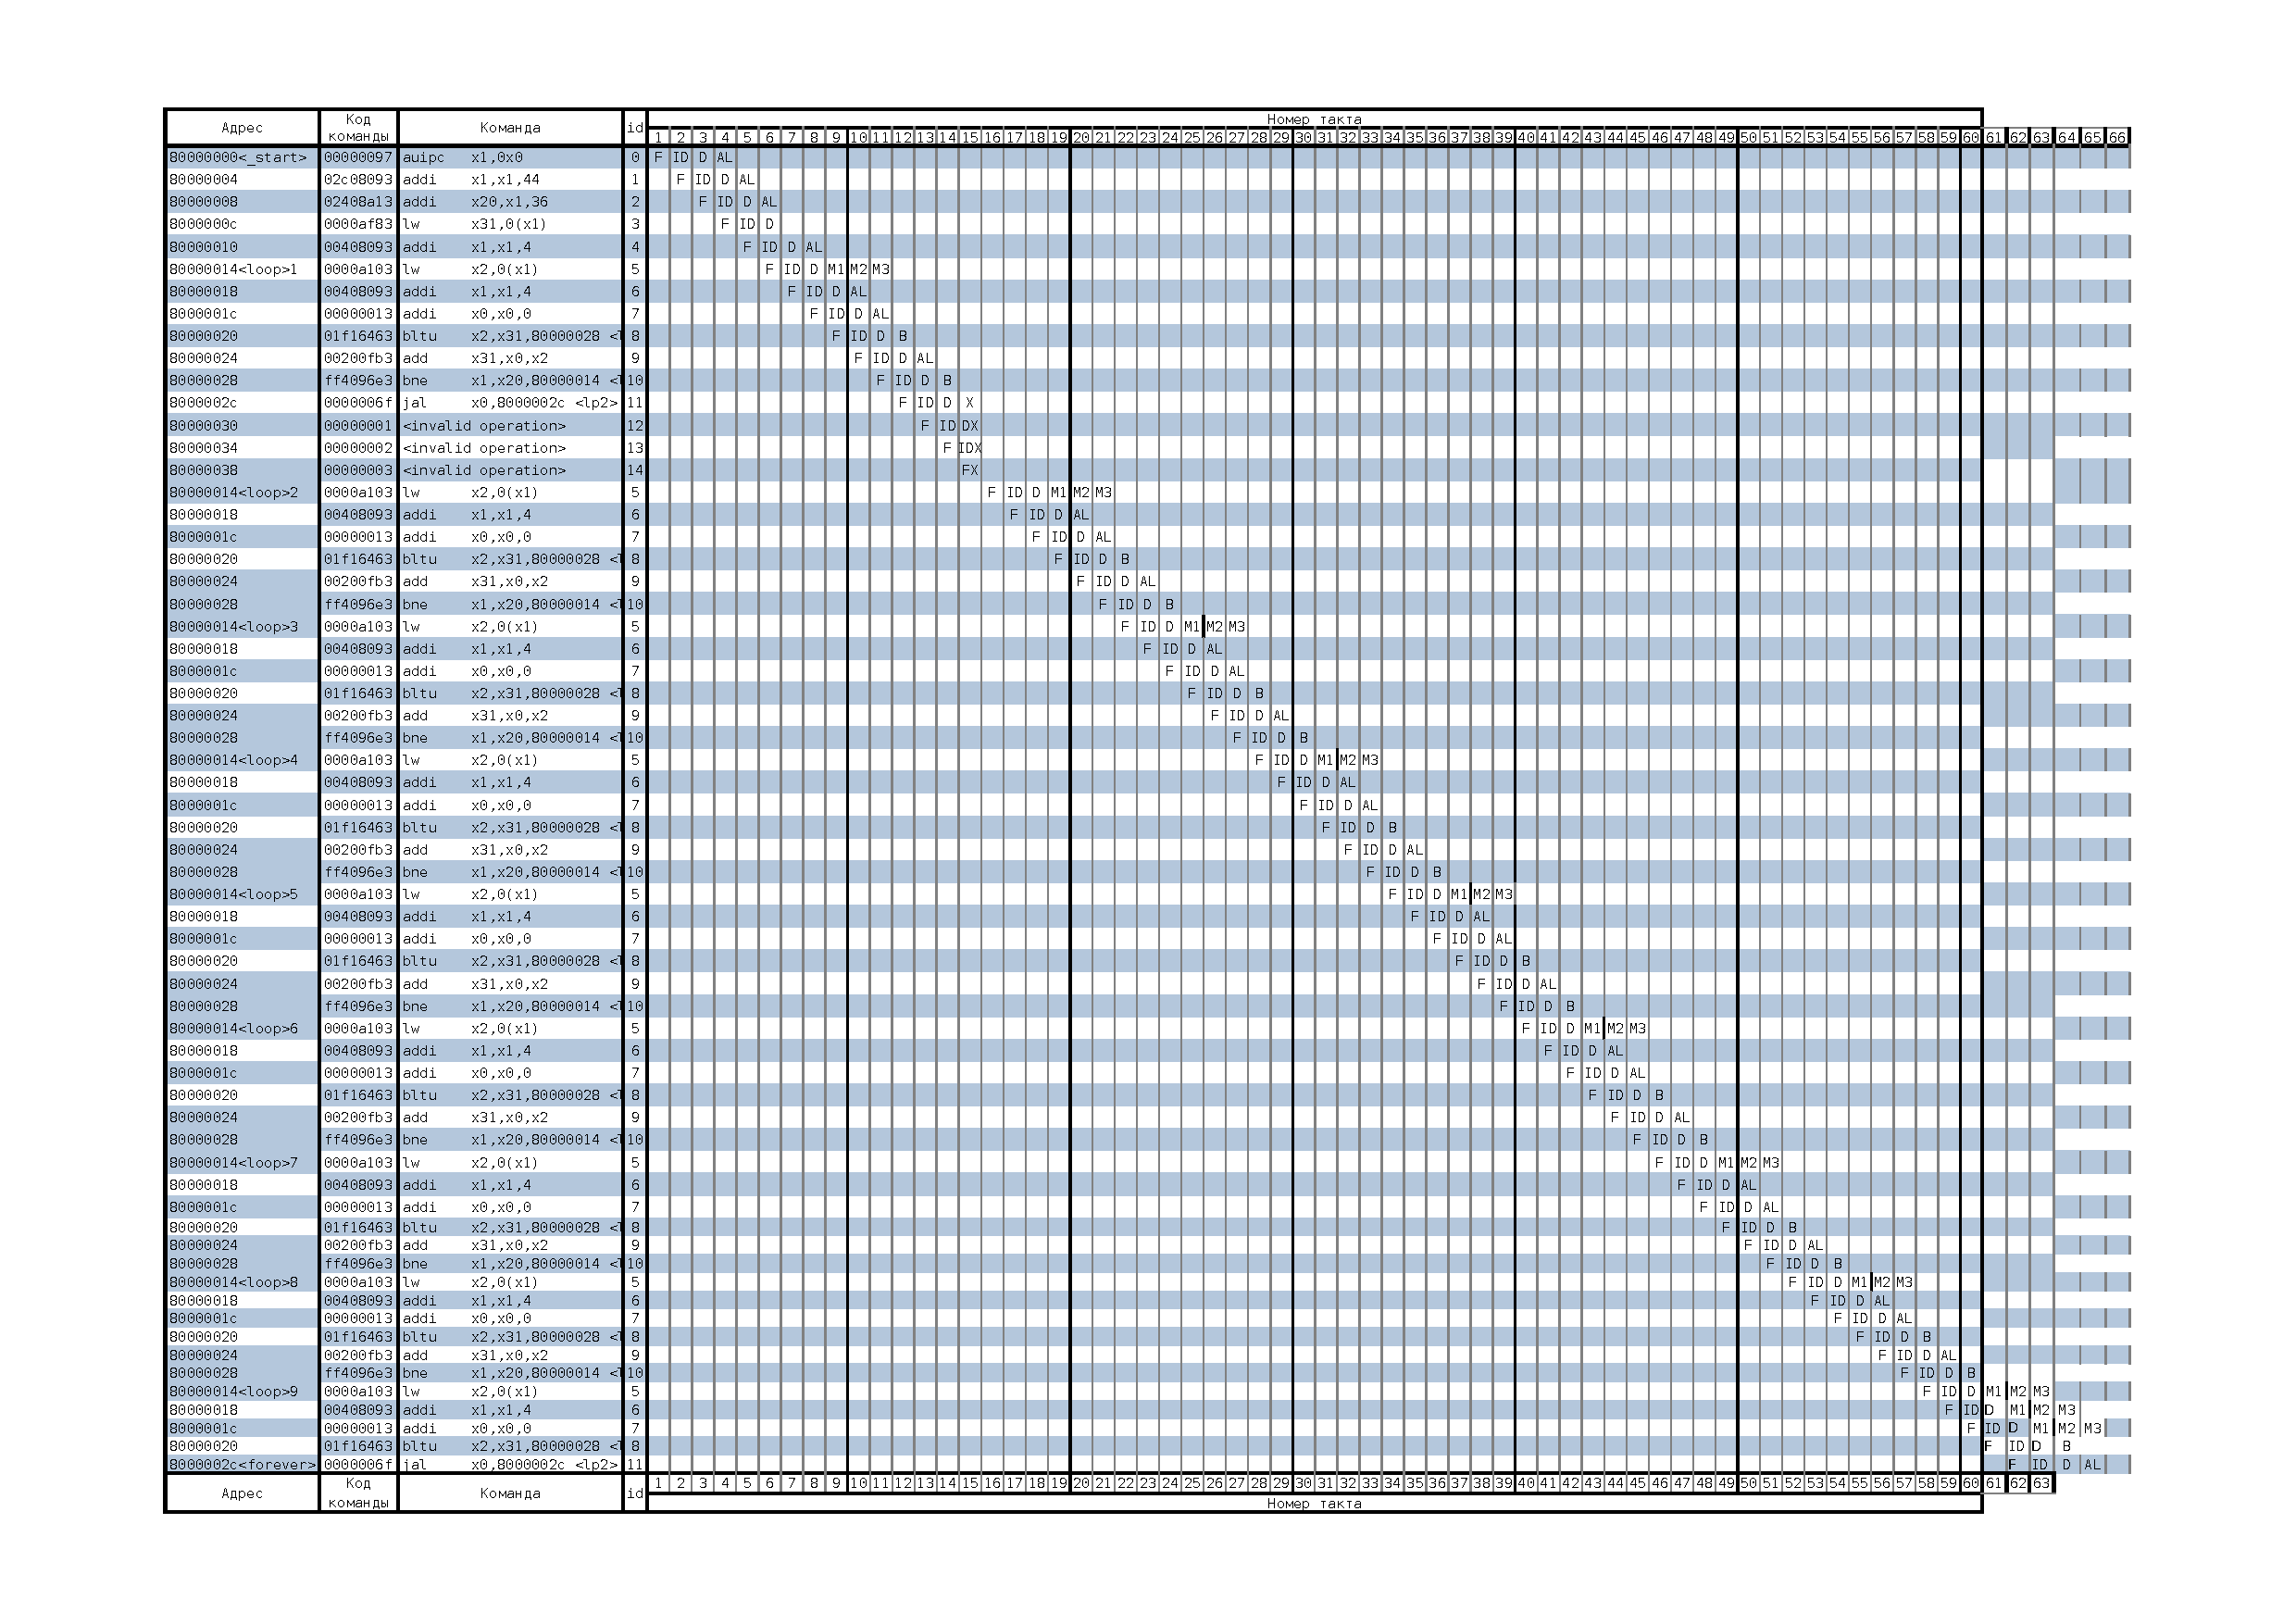
\includegraphics[scale=0.4]{tools/line_opt.pdf}
          \caption{Трасса выполнения оптимизированной программы}
\end{figure}

Можно заметить, что конфликтов больше нет, а трасса стала на 10 такта короче (на 15\%).

\section{Вывод}
В результате данной работы были изучены принципы функционирования, построения и особенности архитектуры 
суперскалярных конвейерных микропроцессоров.

На основе изученных материалов удалось оптимизировать программу.
\end{document}